\subsection{稳健回归}\label{sec:12.4}
如\autoref{sec:10.2}，现在考察基础模型不正确时所用方法的表现，并研究最小二乘估计的一些稳健替代方法，先作一个类似于均值与中位数的比较.

回顾观测$x_1,x_2,\ldots,x_n$时，可将均值和中位数定义为以下量的最小化点：
$$\text{均值：}\min_m\left\{\sum_{i=1}^n(x_i-m)^2\right\},\qquad
\text{中位数：}\min_m\left\{\sum_{i=1}^n|x_i-m|\right\}.$$
对于简单线性回归，观测$(y_1,x_1),\allowbreak(y_2,x_2),\allowbreak\ldots,\allowbreak(y_n,x_n)$，最小二乘回归估计满足
$$\text{最小二乘：}\min_{a,b}\left\{\sum_{i=1}^n[y_i-(a+bx_i)]^2\right\},$$
类似地，定义最小绝对偏差（least absolute deviation，LAD）回归估计为\index{SI0894@最小绝对偏差}\semanticindexanchor{894:514}
$$\text{最小绝对偏差：}\min_{a,b}\left\{\sum_{i=1}^n|y_i-(a+bx_i)|\right\}.$$
（LAD估计可能不唯一，见\autoref{exercise:12.25}.）

可见，最小二乘估计量是样本均值在回归中的对应物. 因此，应当考察它们在\autoref{sec:10.2}第\hyperref[item:10.2.huber.1]{(1)}至\hyperref[item:10.2.huber.3]{(3)}项所列意义下的稳健性表现.

\sourcepageanchor{515}
\begin{example}[最小二乘估计的稳健性]\label{ex:12.4.1}
若观测$(y_1,x_1),\allowbreak(y_2,x_2),\allowbreak\ldots,\allowbreak(y_n,x_n)$，其中
$$Y_i=\alpha+\beta x_i+\varepsilon_i,$$
各$\varepsilon_i$互不相关，$E\varepsilon_i=0$、$\operatorname{Var}\varepsilon_i=\sigma^2$，则已知最小二乘估计量$b$的方差为$\sigma^2/\sum(x_i-\bar x)^2$，是$\beta$的BLUE，满足\autoref{sec:10.2}的第\hyperref[item:10.2.huber.1]{(1)}项.

为考察小偏离下$b$的表现，假定
$$\operatorname{Var}(\varepsilon_i)=\begin{cases}\sigma^2,&\text{概率为 }1-\delta,\\\tau^2,&\text{概率为 }\delta.\end{cases}$$
写$b=\sum d_iY_i$，其中$d_i=(x_i-\bar x)/\sum(x_i-\bar x)^2$，现在有
$$\operatorname{Var}(b)=\sum_{i=1}^nd_i^2\operatorname{Var}(\varepsilon_i)
=\frac{(1-\delta)\sigma^2+\delta\tau^2}{\sum_{i=1}^n(x_i-\bar x)^2}.$$
这说明，和样本均值一样，小扰动下$b$表现相当好. （当然，例如用Cauchy的pdf污染，仍可使情况失控.）最小二乘截距$a$的表现类似（\autoref{exercise:12.22}）. 偏倚污染的影响另见\autoref{exercise:12.23}.
\end{example}

接下来考察一个“灾难性”观测的影响，并将最小二乘与对应于中位数的替代方法——最小绝对偏差回归——比较.

\begin{example}[灾难性观测]\label{ex:12.4.2}
\hyperref[bib:source217]{McPherson（1990）}描述了一项实验，测量24只长鼻袋鼠（potoroo，一种有袋动物）育儿袋中的二氧化碳（$\mathrm{CO}_2$）和氧气（$\mathrm O_2$）浓度. 关心$\mathrm{CO}_2$对$\mathrm O_2$的回归，实验者预期斜率为$-1$. 23只动物的数据见\autoref{tab:12.4.2}，另一只有缺失值. 对原始数据，最小二乘与LAD直线很接近：
$$\begin{aligned}\text{最小二乘}&:\quad y=18.67-0.89x,\\
\text{最小绝对偏差}&:\quad y=18.59-0.89x.
\end{aligned}$$
然而，异常观测可能扰乱最小二乘. 输入数据时，第15只动物的$\mathrm O_2$值18被错录为10，我们确实这样做了. 对这一新的错误数据集，有
$$\begin{aligned}\text{最小二乘}&:\quad y=6.41-0.23x,\\
\text{最小绝对偏差}&:\quad y=15.95-0.75x,
\end{aligned}$$
说明异常观测对LAD的影响小得多. 回归直线见\autoref{fig:12.4.1}.

这些计算说明，与最小二乘相比，LAD具有抵抗性. 由于均值与中位数的类比，可以推测这种表现反映在崩溃值中：最小二乘为0\%，LAD为50\%.\footnote{译注：回归LAD的崩溃值不能一般地照搬中位数的50\%；若允许污染预测变量$x$，单个高杠杆点也可使LAD斜率失控. 上述数值须有额外污染范围和设计条件，原文未列明，照录.}
\end{example}

不过，均值与中位数的类比仍在继续. 虽然LAD估计量能稳健地对待灾难性观测，但相对于最小二乘估计量，它损失了很多效率（另见\autoref{exercise:12.25}）.

\begin{example}[LAD估计量的渐近正态性]\label{ex:12.4.3}
调整推导\eqref{eq:10.2.6}的论证，求LAD估计量的渐近分布. 为简化，仅考虑模型
$$Y_i=\beta x_i+\varepsilon_i,$$
即令$\alpha=0$，从而避免处理二元极限分布.

\sourcepageanchor{516}
\begin{table}[htbp]\centering
\setcounter{table}{1}
\caption{23只长鼻袋鼠育儿袋中的$\mathrm{CO}_2$与$\mathrm O_2$值（\hyperref[bib:source217]{McPherson，1990）}}\label{tab:12.4.2}
\begin{tabular}{lrrrrrrrr}\toprule
动物&1&2&3&4&5&6&7&8\\\midrule
$\%\,\mathrm O_2$&20&19.6&19.6&19.4&18.4&19&19&18.3\\
$\%\,\mathrm{CO}_2$&1&1.2&1.1&1.4&2.3&1.7&1.7&2.4\\\midrule
动物&9&10&11&12&13&14&15&16\\\midrule
$\%\,\mathrm O_2$&18.2&18.6&19.2&18.2&18.7&18.5&18&17.4\\
$\%\,\mathrm{CO}_2$&2.1&2.1&1.2&2.3&1.9&2.4&2.6&2.9\\\midrule
动物&17&18&19&20&21&22&23&\\\midrule
$\%\,\mathrm O_2$&16.5&17.2&17.3&17.8&17.3&18.4&16.9&\\
$\%\,\mathrm{CO}_2$&4.0&3.3&3.0&3.4&2.9&1.9&3.9&\\\bottomrule
\end{tabular}
\end{table}
\begin{figure}[htbp]\centering
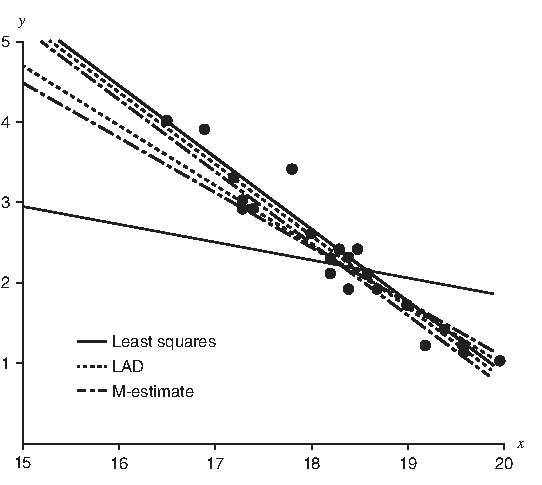
\includegraphics[width=.75\textwidth]{assets/chapter12/fig-12.4.1.pdf}
\caption{\autoref{tab:12.4.2}数据的最小二乘、LAD及M估计拟合，分别使用原始数据与将$(18,2.6)$误录为$(10,2.6)$的数据. LAD与M估计直线十分相似，而最小二乘直线会对数据变化作出反应.}\label{fig:12.4.1}
\end{figure}
用M估计量的术语说，LAD估计量由最小化下式得到：
\begin{equation}\label{eq:12.4.1}
\begin{aligned}
\sum_{i=1}^n\rho(y_i-\beta x_i)&=\sum_{i=1}^n|y_i-\beta x_i|\\
&=\sum_{i=1}^n\bigl[(y_i-\beta x_i)I(y_i>\beta x_i)-(y_i-\beta x_i)I(y_i<\beta x_i)\bigr].
\end{aligned}
\end{equation}
然后计算$\psi=\rho'$，求解$\sum_i\psi(y_i-\beta x_i)=0$得到$\beta$，其中\footnote{译注：原文$\psi=\rho'$与随后含$x_i$的式子并非同一变量下的导数；后式实际是目标函数对$\beta$的负导数所对应的加权符号函数，并在残差为零处不可微. 原表述保留.}
$$\psi(y_i-\beta x_i)=x_iI(y_i>\beta x_i)-x_iI(y_i<\beta x_i).$$

\sourcepageanchor{517}
若$\hat\beta_L$是解，在$\beta$附近将$\psi$展开为Taylor级数：
$$\begin{aligned}
\sum_{i=1}^n\psi(y_i-\hat\beta_Lx_i)
&=\sum_{i=1}^n\psi(y_i-\beta x_i)\\
&\quad+(\hat\beta_L-\beta)\left.\frac d{d\hat\beta_L}\sum_{i=1}^n\psi(y_i-\hat\beta_Lx_i)\right|_{\hat\beta_L=\beta}+\cdots.
\end{aligned}$$
虽然等式左边不等于零，假定它在$n\to\infty$时趋于零（见\autoref{exercise:12.27}）. 重新整理得
\begin{equation}\label{eq:12.4.2}
\sqrt n(\hat\beta_L-\beta)=
\frac{-\dfrac1{\sqrt n}\sum_{i=1}^n\psi(y_i-\beta x_i)}
{\left.\dfrac1n\dfrac d{d\hat\beta_L}\sum_{i=1}^n\psi(y_i-\hat\beta_Lx_i)\right|_{\hat\beta_L=\beta}}.
\end{equation}
先看分子. 因为$E_\beta\psi(Y_i-\hat\beta_Lx_i)=0$且$\operatorname{Var}\psi(Y_i-\hat\beta_Lx_i)=x_i^2$，有\footnote{译注：这些均值、方差应在真实参数$\beta$处计算，并需误差中位数为零等条件；原文此处写估计量$\hat\beta_L$，下一式又写$\hat\beta$，与\eqref{eq:12.4.2}分子的$\beta$不一致. 原符号均保留.}
\begin{equation}\label{eq:12.4.3}
-\frac1{\sqrt n}\sum_{i=1}^n\psi(Y_i-\hat\beta x_i)
=\sqrt n\left[-\frac1n\sum_{i=1}^n\psi(Y_i-\hat\beta x_i)\right]
\to\mathrm n(0,\sigma_x^2),
\end{equation}
其中$\sigma_x^2=\lim_{n\to\infty}\frac1n\sum_{i=1}^nx_i^2$. 转向分母，因为$\psi$有不可微点，必须小心. 因此，先应用大数定律，再求导，并采用近似
\begin{equation}\label{eq:12.4.4}
\begin{aligned}
\frac1n\frac d{d\beta_0}\sum_{i=1}^n\psi(y_i-\beta_0x_i)
&\approx\frac1n\sum_{i=1}^n\frac d{d\beta_0}E_\beta[\psi(Y_i-\beta_0x_i)]\\
&=\frac1n\sum_{i=1}^n\frac d{d\beta_0}\bigl[x_iP_\beta(Y_i>\beta_0x_i)-x_iP_\beta(Y_i<\beta_0x_i)\bigr]\\
&=\frac1n\sum_{i=1}^n\bigl[x_i^2f(\beta_0x_i-\beta x_i)+x_i^2f(\beta_0x_i-\beta x_i)\bigr].
\end{aligned}
\end{equation}
在$\beta_0=\beta$处计算导数，得\footnote{译注：按上文$\psi$的符号约定，对两个概率求导后均应带负号，故\eqref{eq:12.4.4}最后一行及此近似右端应为负；最终方差使用平方，不受这一符号影响. 原式保留.}
$$\left.\frac1n\frac d{d\beta_0}\sum_{i=1}^n\psi(y_i-\beta_0x_i)\right|_{\beta_0=\beta}
\approx2f(0)\frac1n\sum_{i=1}^nx_i^2,$$
结合\eqref{eq:12.4.2}、\eqref{eq:12.4.3}，有
\begin{equation}\label{eq:12.4.5}
\sqrt n(\hat\beta_L-\beta)\to\mathrm n\left(0,\frac1{4f(0)^2\sigma_x^2}\right).
\end{equation}
最后，$\alpha=0$时最小二乘估计量为$\hat\beta=\sum_{i=1}^nx_iy_i/\sum_{i=1}^nx_i^2$，满足
$$\sqrt n(\hat\beta-\beta)\to\mathrm n\left(0,\frac1{\sigma_x^2}\right),$$
所以$\hat\beta_L$相对于$\hat\beta$的渐近相对效率为
$$\operatorname{ARE}(\hat\beta_L,\hat\beta)=\frac{1/\sigma_x^2}{1/(4f(0)^2\sigma_x^2)}=4f(0)^2,$$
其值与\autoref{tab:10.2.2}中中位数相对于均值的值相同. 因此，对正态误差，LAD估计量相对于最小二乘的ARE只有64\%，说明LAD牺牲了相当多的效率.\footnote{译注：这里的最小二乘极限方差及ARE采用误差方差为1的标准化；一般误差方差$\sigma^2$下，应分别为$\sigma^2/\sigma_x^2$与$4\sigma^2f(0)^2$. 原式未明示此标准化，照录.}
\end{example}
\sourcepageanchor{518}
于是又遇到\autoref{sec:10.2.1}的情形：若误差确为正态，以LAD代替最小二乘似乎损失了过多效率. 折中方法仍然是M估计量. 可以最小化类似\eqref{eq:10.2.2}的函数$\sum_i\rho_i(\alpha,\beta)$来构造，其中
\begin{equation}\label{eq:12.4.6}
\rho_i(\alpha,\beta)=\begin{cases}
\tfrac12(y_i-\alpha-\beta x_i)^2,&|y_i-\alpha-\beta x_i|\le k,\\
k|y_i-\alpha-\beta x_i|-\tfrac12k^2,&|y_i-\alpha-\beta x_i|\ge k,
\end{cases}
\end{equation}
$k$为调节参数.

\begin{example}[回归M估计量]\label{ex:12.4.4}
使用\eqref{eq:12.4.6}，取$k=1.5\sigma$，对\autoref{tab:12.4.2}的数据拟合$\alpha,\beta$的M估计量，结果为
$$\begin{aligned}\text{原始数据的M估计}&:\quad y=18.5-0.89x,\\
\text{误录数据的M估计}&:\quad y=14.67-0.68x,
\end{aligned}$$
其中以最小二乘拟合残差的标准差.23估计$\sigma$.

可见，M估计比最小二乘直线更有抵抗性，有离群值时的表现更像LAD拟合.
\end{example}

如\autoref{sec:10.2}，预期M估计量的ARE优于LAD. 确实如此，但计算变得十分复杂，比LAD还复杂，因此不在这里给出细节. \hyperref[bib:source171]{Huber（1981}，第7章）详细讨论了M估计量的渐近理论，另见\hyperref[bib:source243]{Portnoy（1987）}. 这里满足于通过一个小型模拟研究评价M估计量，重现类似\autoref{tab:10.2.4}的表.

\begin{example}[回归ARE的模拟]\label{ex:12.4.5}
对于模型$Y_i=\alpha+\beta x_i+\varepsilon_i$，$i=1,2,\ldots,5$，取$x_i$为$(-2,-1,0,1,2)$，$\alpha=0$、$\beta=1$. 从正态、双指数和Laplace分布生成$\varepsilon_i$，计算最小二乘、LAD和M估计量的方差，列于\autoref{tab:12.4.3}.\footnote{译注：双指数分布与Laplace分布通常是同一分布；原文列举与表中“正态、Logistic、双指数”不一致，可能将Logistic误写为Laplace. 原文照录.}
\begin{table}[htbp]\centering
\caption{回归M估计量的渐近相对效率，$k=1.5$（基于10,000次模拟）}\label{tab:12.4.3}
\begin{tabular}{lrrr}\toprule
&正态&Logistic&双指数\\\midrule
相对于最小二乘&0.98&1.03&1.07\\
相对于LAD&1.39&1.27&1.14\\\bottomrule
\end{tabular}
\end{table}
三种分布下，M估计量的方差都与最小二乘相近，并且都优于LAD. M估计量相对于LAD的优势，比\autoref{tab:10.2.4}中Huber估计量相对于中位数的优势更显著.
\end{example}
